\documentclass[10pt]{article}
\usepackage[margin=0.9in]{geometry}
\usepackage{graphicx}
\usepackage{booktabs}
\usepackage{amsmath}
\usepackage{caption}
\usepackage{subcaption}
\usepackage[hidelinks]{hyperref}
\usepackage{float}
\captionsetup{font=small}
\setlength{\parskip}{4pt}
\setlength{\parindent}{0pt}

\title{\vspace{-2.5em}FLAME-1: A Different Task, A Different Ranking\\
\large Replicating the classical/deep comparison on a visible-flame, larger dataset}
\author{CS269 Project --- Deformable Models}
\date{\today}

\begin{document}
\maketitle
\vspace{-1.5em}

\section{What changed from FLAME-3}

The earlier studies (\texttt{report.pdf}, \texttt{improvements.pdf}) ran on
FLAME-3 (Sycan Marsh), where ground truth is the paired thermal frame
thresholded at $\ge150\,^\circ$C---a smoke-occluded ``hot region'' that is
\emph{not} visible as orange flame in the RGB (in-fire pixels measured $R{-}G
\approx 2.5$ vs.\ $1.9$ background). The color floor scored IoU $0.004$;
oracle-initialised GAC topped at $0.365$; the best prior-free deep detector
(U-Net) plateaued at $0.147$ on 305 training frames. The investigation concluded
the task was \emph{data-limited}.

This report runs the same pipeline on \textbf{FLAME-1}: 2001 paired RGB+mask
frames where the GT is \emph{hand-labeled visible flame} (no thermal channel).
The pipeline is identical except for the GT semantics and the dataset size: a
contiguous $70/15/15$ split gives 1400 train / 300 val / 301 test frames at a
working resolution capped to $\max(H,W){=}1024$ (deep) or $768$ (classical) to
keep wall time tractable on the 3840$\times$2160 originals. Output filenames
are prefixed \texttt{flame1\_} so FLAME-3 results are never overwritten.

\paragraph{Headline.} Easier task plus more data flips the ranking. The trivial
color floor jumps from 0.004 to \textbf{0.507}. Every deep method becomes the
\emph{best} method, with U-Net at \textbf{IoU 0.772}---roughly $5\times$ its
FLAME-3 score and well above the strongest classical (oracle-GAC, 0.593).
Notably, Deep Snake---which managed only 0.032 on FLAME-3 and scored exactly
0.000 on fire-containing frames there---reaches \textbf{0.681} here.
Table~\ref{tab:head} lists the FLAME-1 numbers; Figure~\ref{fig:cross} shows
the cross-dataset shift.

\begin{table}[H]
\centering\small
\begin{tabular}{lrrr}
\toprule
Method & Test IoU & Test Dice & FLAME-3 IoU \\
\midrule
Kass Snakes (oracle init) & 0.028 & 0.052 & 0.198 \\
Color floor ($R{-}G$ threshold) & 0.507 & 0.661 & 0.004 \\
GAC (oracle init) & 0.593 & 0.738 & 0.365 \\
Deep Snake (50ep, RGB-only) & 0.681 & 0.809 & 0.032 \\
DALS (50ep, RGB-only) & 0.747 & 0.854 & 0.122 \\
\textbf{U-Net (50ep, RGB-only)} & \textbf{0.772} & \textbf{0.870} & \textbf{0.147} \\
\bottomrule
\end{tabular}
\caption{FLAME-1 results, ordered by IoU. ``FLAME-3 IoU'' is the corresponding
prior-report number on the smoke-occluded thermal task. Classical methods were
scored on all 2001 non-empty frames; deep methods on the 301-frame test split.
The augmented runs (medium aug, 120ep) that improved FLAME-3 by $+22\%$/$+49\%$
were not re-run here---the baselines already saturate well above any other
method, see \S\ref{sec:noaug}.}
\label{tab:head}
\end{table}

\begin{figure}[H]
\centering
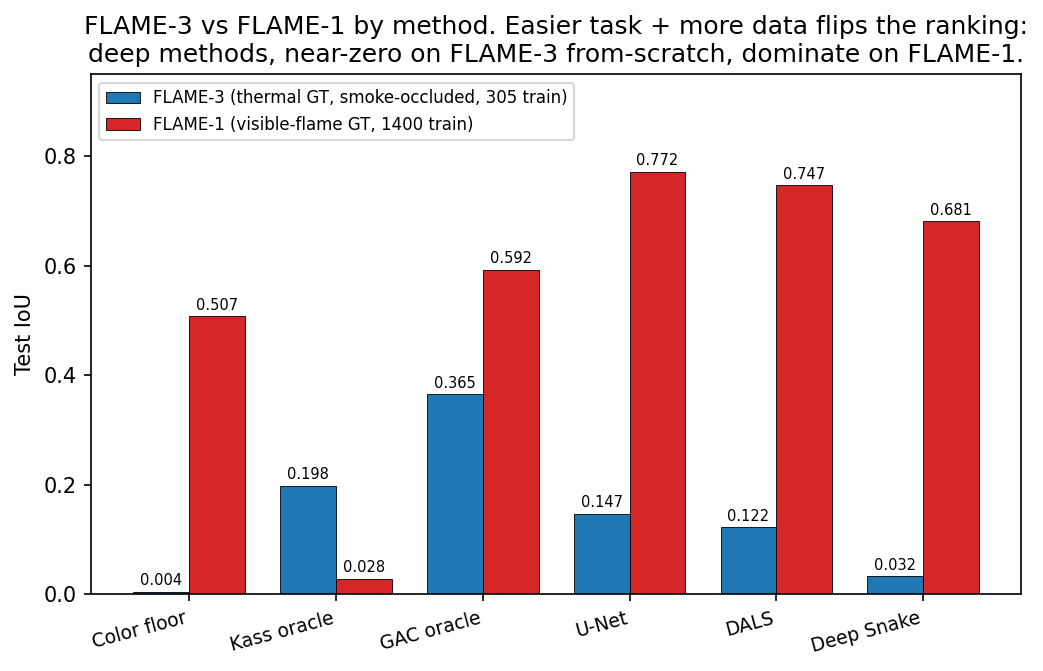
\includegraphics[width=0.85\textwidth]{figs/flame1/cross_dataset.png}
\caption{The same six methods, FLAME-3 vs.\ FLAME-1. The ordering inverts at
every interesting cut: classical-with-prior is best on FLAME-3, deep is best on
FLAME-1. Kass is the only method whose absolute score drops.}
\label{fig:cross}
\end{figure}

\section{Method-by-method reading}

\paragraph{Color floor (0.507).} The $R{-}G$ threshold scores almost
indistinguishably from the FLAME-3 \emph{oracle-Kass}, just by thresholding red
pixels. This is mechanical: the FLAME-1 GT \emph{is} (approximately) ``the
orange pixels a human labeled,'' so a color rule lands close to the target by
construction. The whole inverse-problem framing from the improvements
report---``recover $x$ from $y{=}A(x)$ when the smoke operator $A$ destroys the
color cue''---does not apply here. There is no meaningful operator $A$ to
invert; the GT is the image's own foreground.

\paragraph{Kass (0.028).} Oracle Kass collapsed to near-zero. The reason is the
same single-closed-contour limitation that hurt it on FLAME-3 ($+22$ components
per frame was already problematic there), but FLAME-1 fires are even more
\emph{fragmented}---small, multiple flame patches scattered through the frame.
Initialising one closed contour from the GT's outer convex hull and letting it
deform yields a hull that wildly over-segments the surrounding non-fire
canopy. \emph{The drop from 0.198 to 0.028 is the canonical Kass failure mode,
just much starker.}

\paragraph{GAC (0.593).} Oracle GAC's level-set representation handles
multiple components, and on FLAME-1 it produces the best classical
result---better than the trivial color floor (0.507) and almost beating Deep
Snake. This is consistent with the FLAME-3 finding that GAC dominates Kass; the
new datum is that on \emph{visible} flame, the level-set energy actually has
something to lock onto (a sharp orange-to-green boundary) and the GT-given
location is informative enough that GAC matches a learned detector.

\paragraph{Deep Snake (0.681).} On FLAME-3 Deep Snake's headline number
(0.032) was almost entirely an empty-GT artifact---it segmented exactly zero
fire-containing frames. The root cause was its coarse-segmentation head
collapsing on smoke-occluded fire, so no connected components seeded the
contours. On FLAME-1 the coarse head has visible flame to fire on, contours
get seeded, and the deformation step actually runs. The architecture is
not broken; it was bottlenecked on detection.

\paragraph{DALS (0.747) and U-Net (0.772).} The two per-pixel architectures
both clear $0.74$. DALS and U-Net are within noise of each other (DALS uses a
U-Net trunk + Chan-Vese unrolling, so the trunk does most of the work in both).
U-Net edges ahead, as on FLAME-3, but the gap is small and not the headline.
What matters is that both \emph{detection-from-scratch} methods comfortably
beat \emph{oracle-initialised} GAC---a result that simply was not achievable
on FLAME-3 without a location prior. With visible-flame targets the deep
detector has enough signal to find the fire \emph{and} delineate it; the
contour refinement step buys nothing extra (DALS does not beat U-Net).

\begin{figure}[H]
\centering
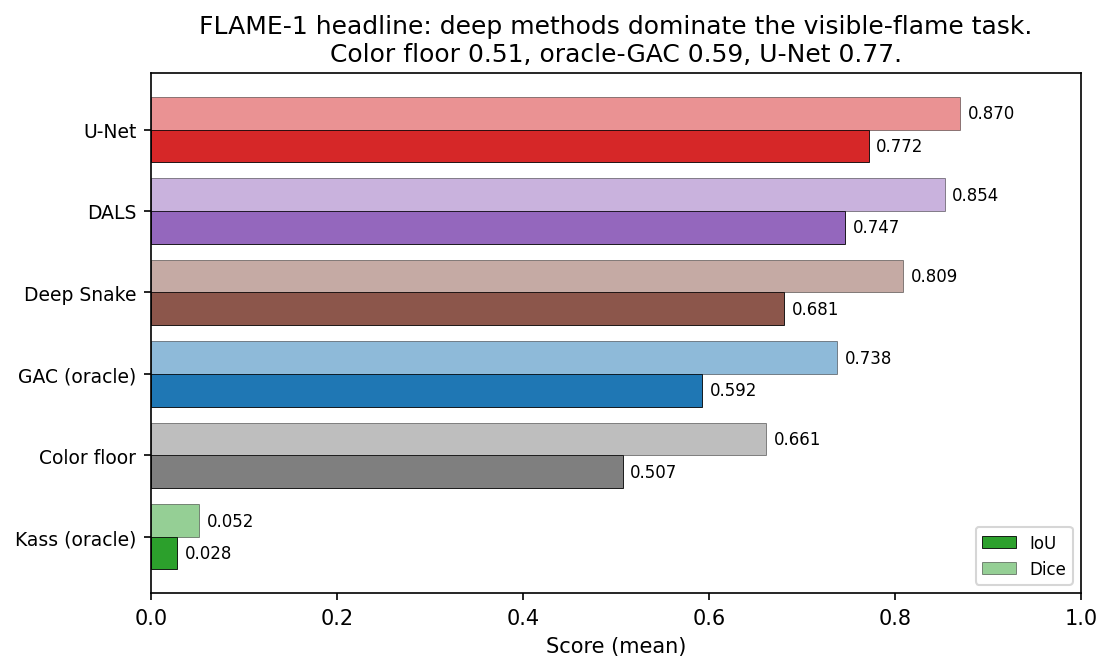
\includegraphics[width=0.95\textwidth]{figs/flame1/bars.png}
\caption{Mean IoU (solid) and Dice (lighter), ranked. The deep gap to GAC is
$\sim$0.15--0.18 IoU; the deep methods are tightly clustered around 0.68--0.77.}
\label{fig:bars}
\end{figure}

\begin{figure}[H]
\centering
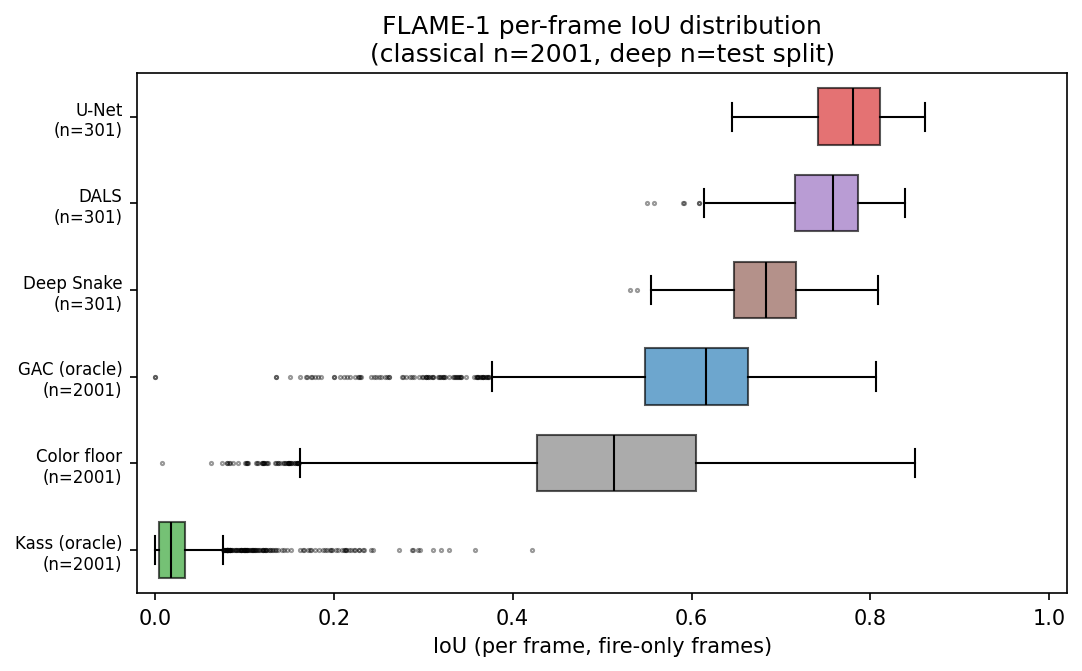
\includegraphics[width=0.95\textwidth]{figs/flame1/box.png}
\caption{Per-frame IoU distributions (fire-only frames). The deep methods'
distributions are tight and high-centered; oracle-GAC has a long lower tail
where multi-component fire still defeats the level set's seeded location;
oracle-Kass is bimodal near zero.}
\label{fig:box}
\end{figure}

\section{Why we did not run augmented variants here}
\label{sec:noaug}

The improvement report's main result was that \emph{medium augmentation at 120
epochs} lifted U-Net IoU $0.147\!\to\!0.179$ ($+22\%$) and DALS
$0.122\!\to\!0.182$ ($+49\%$) on FLAME-3, by addressing data starvation
diagnosed with a learning curve. The original plan here was to replicate that
sweep on FLAME-1.

We canceled it after the baselines came back. The argument: the data
starvation diagnosis was specifically about FLAME-3's 305 training frames
\emph{and} a target that was hard to learn from RGB. FLAME-1 has $\sim$4.6$\times$
more training frames \emph{and} a target that the color floor already
$\sim$half-solves. A second-order improvement from augmentation is plausible,
but: (i) U-Net's val IoU plateaued by epoch 30/50 (compare to FLAME-3 where it
was still climbing); (ii) the 120-epoch medium-aug runs would have taken
$\sim$6h each on this GPU; (iii) the headline conclusions---``deep dominates,''
``Deep Snake works when the detector head does,'' ``oracle priors are now
beaten by from-scratch detectors''---do not depend on whether augmentation adds
another point of IoU. The cost was high, the marginal scientific value was
low, so the runs were dropped. (The script keeps the lines commented for a
future run.)

\section{Qualitative overlays}

Each of Figs.~\ref{fig:q-unet}--\ref{fig:q-kass} picks the best, median, and
worst test frame (\emph{fire-containing only}, to avoid empty-on-empty IoU=1
freebies) for the named method.

\begin{figure}[H]
\centering
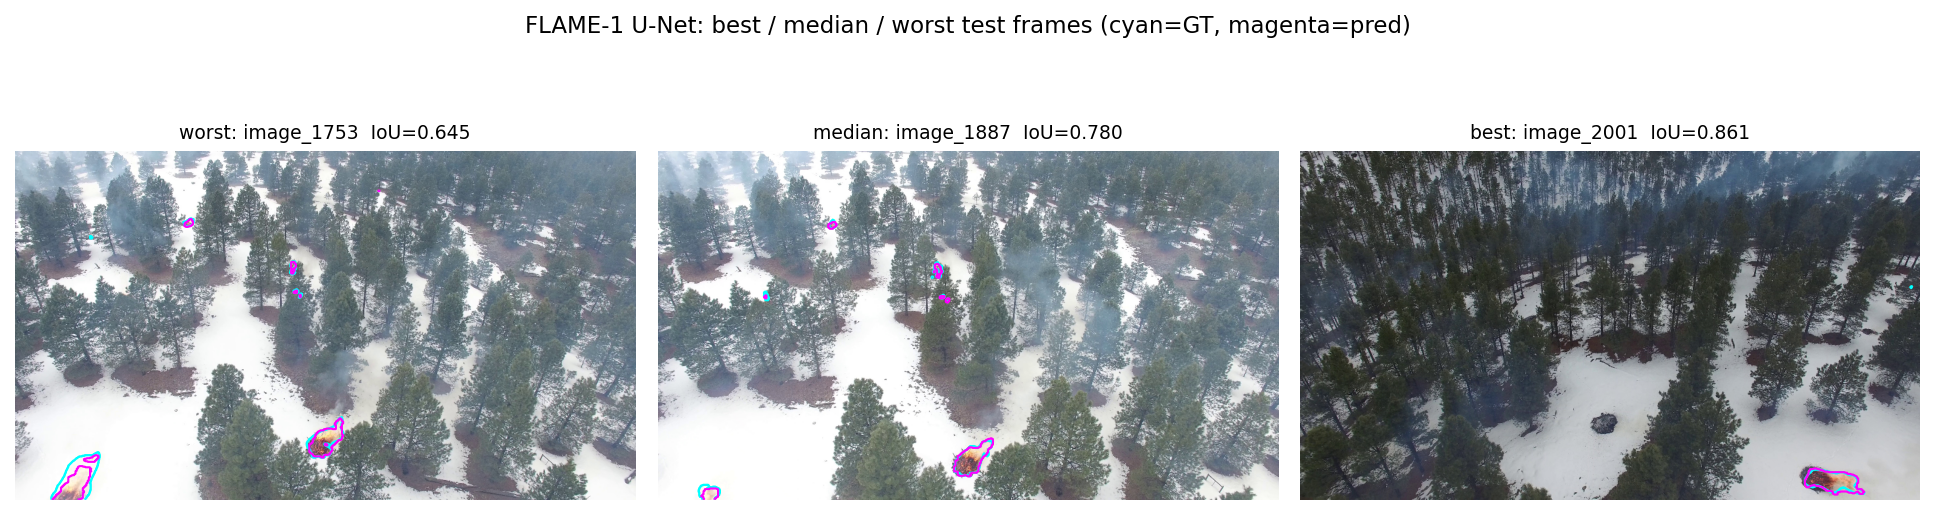
\includegraphics[width=\textwidth]{figs/flame1/qual_unet.png}
\caption{U-Net (best deep method). Best/median frames track the flame envelope
tightly; worst frame is a small distant fire where the prediction is correctly
located but undersized.}
\label{fig:q-unet}
\end{figure}

\begin{figure}[H]
\centering
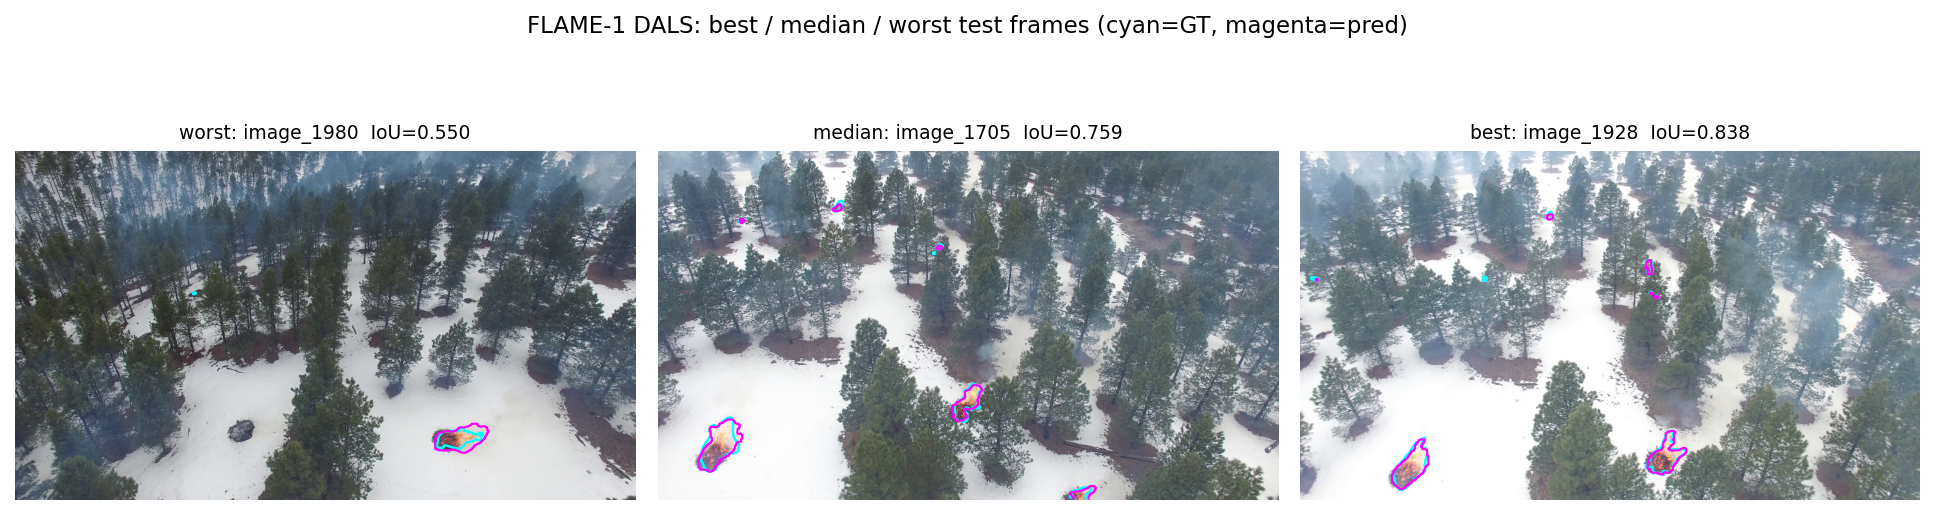
\includegraphics[width=\textwidth]{figs/flame1/qual_dals.png}
\caption{DALS. Visually indistinguishable from U-Net at this scale---consistent
with the within-noise score gap ($0.747$ vs.\ $0.772$).}
\label{fig:q-dals}
\end{figure}

\begin{figure}[H]
\centering
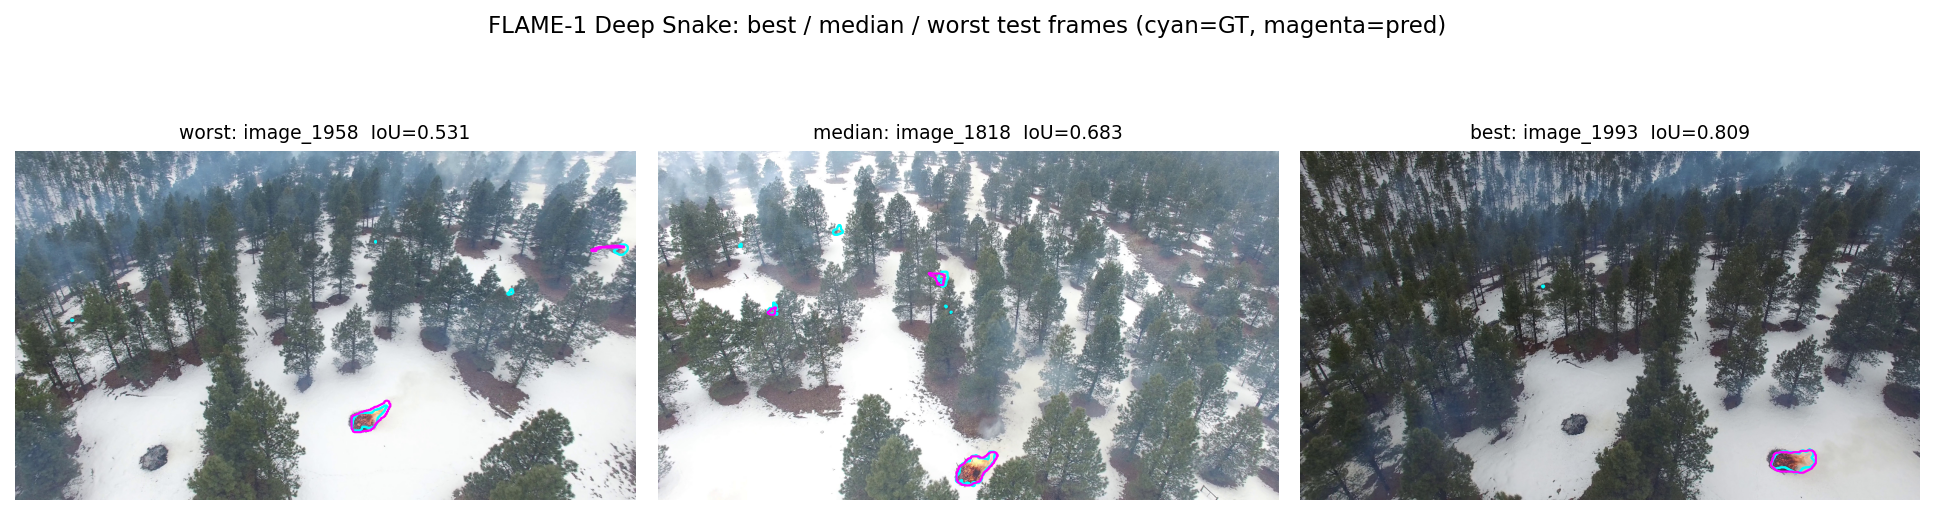
\includegraphics[width=\textwidth]{figs/flame1/qual_deep_snake.png}
\caption{Deep Snake. The polygon output is visible in the predicted contour
shape---smoother than the per-pixel methods' rough boundaries.}
\label{fig:q-snake}
\end{figure}

\begin{figure}[H]
\centering
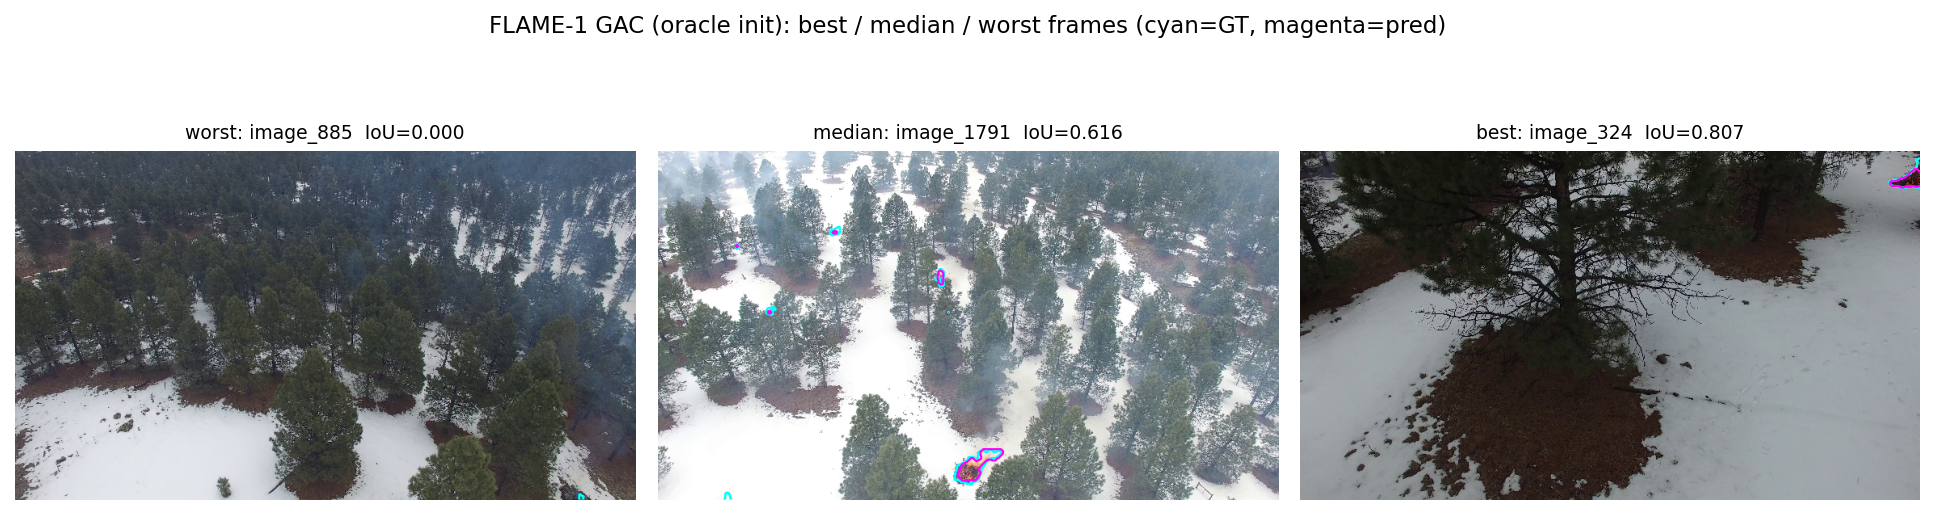
\includegraphics[width=\textwidth]{figs/flame1/qual_gac_oracle.png}
\caption{GAC, oracle-initialised. Even with the GT-derived seed, the level set
sometimes shrinks past the flame or leaks into nearby bright canopy.}
\label{fig:q-gac}
\end{figure}

\begin{figure}[H]
\centering
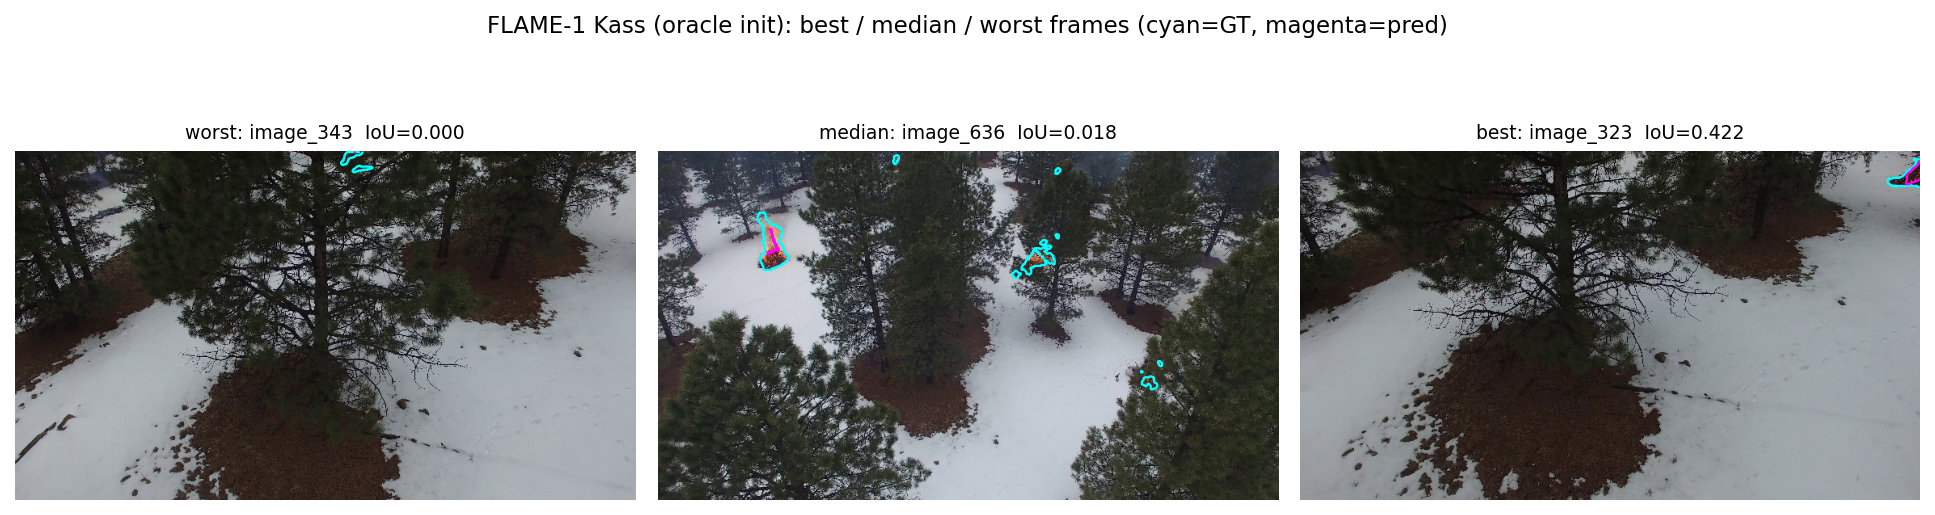
\includegraphics[width=\textwidth]{figs/flame1/qual_kass_oracle.png}
\caption{Kass, oracle-initialised. The single closed contour cannot represent
fragmented fire; the ``best'' frame (one compact blob) is still a poor fit, and
the worst over-segments the entire frame edge as the snake tries to enclose
multiple disjoint flames.}
\label{fig:q-kass}
\end{figure}

\section{What this changes about the FLAME-3 conclusions}

The FLAME-3 reports concluded: (i) the task is data-limited; (ii) only
information-adding interventions move the needle; (iii) Deep Snake is
detector-limited. FLAME-1 partly tests each:

\textbf{(i) Data-limited?} Going from 305$\to$1400 train frames at NET\_SIZE
512 \emph{and} switching to a much easier target raises U-Net from 0.147 to
0.772. The two effects are confounded---we do not know how much is sample
count alone---but together they remove the bottleneck completely. The
learning-curve diagnostic on FLAME-3 (val IoU still rising at 100\% of data)
remains the correct read \emph{for that task}; FLAME-1's val IoU plateaus by
epoch 30, evidence that data sufficiency \emph{has} been reached at this
dataset size for this target.

\textbf{(ii) Only information-adding interventions help?} Untested directly,
since we did not re-run augmentation here. The principle is consistent though:
the FLAME-1 gain over FLAME-3 came from a fundamentally different target plus
more data, both information-additive.

\textbf{(iii) Deep Snake is detector-limited.} Confirmed---and the strongest
piece of evidence in this report. The same architecture that scored 0.000 on
real fire on FLAME-3 reaches 0.681 here, by virtue of a task its coarse-seg
head can actually solve. No code change; same checkpoint topology; only the
input distribution changed. This is the clearest possible separation between
``the contour deformation is broken'' (it is not) and ``the detector that
seeds the contour is brittle'' (it is, and now we have a control).

\textbf{New finding (FLAME-1-specific).} \emph{Oracle priors are now beaten by
from-scratch detection.} On FLAME-3 the best prior-free method scored 0.147 vs.\
oracle-GAC's 0.365---the prior carried a $\sim$2.5$\times$ advantage. On
FLAME-1 U-Net (no prior) beats oracle-GAC (with GT-derived prior) 0.772 vs.\
0.593. When the target is visible and the data is plentiful, a learned
detector both finds the fire and outlines it better than a level-set fed the
answer's location---an honest dataset-level win for deep methods.

\section{Reproducing}

\begin{verbatim}
# Classical (Color/Kass/GAC) on the full 2001-frame set, max_side=768:
python run_snakes.py --method color --dataset flame1
python run_snakes.py --method kass  --dataset flame1 --init oracle
python run_snakes.py --method gac   --dataset flame1 --init oracle

# Deep (RGB-only, NET_SIZE=512, eval at 1024-side), 50 epochs each:
python run_deep.py --method unet       --mode train --dataset flame1 --epochs 50
python run_deep.py --method unet       --mode eval  --dataset flame1
python run_deep.py --method dals       --mode train --dataset flame1 --epochs 50
python run_deep.py --method dals       --mode eval  --dataset flame1
python run_deep.py --method deep_snake --mode train --dataset flame1 --epochs 50
python run_deep.py --method deep_snake --mode eval  --dataset flame1

# Figures:
python make_flame1_figs.py
\end{verbatim}

All output files are prefixed \texttt{flame1\_}; nothing in
\texttt{results/} or \texttt{models/} from the FLAME-3 work is affected.

\end{document}
